\documentclass{beamer}

\usepackage[T1]{fontenc}
\usepackage[utf8]{inputenc}
\usepackage[ngerman]{babel}
\usepackage{lmodern}

%\usepackage{geometry}
%\geometry{
%left=20mm,
%right=20mm,
%top=20mm,
%}

\usepackage{amsmath}
\usepackage{amsfonts}
\usepackage{xcolor}
\usepackage{graphicx}
\graphicspath{{img/}{img/ink/}}

\usetheme{Darmstadt}
\usecolortheme{crane}

\title{Phyphox}

\setbeamertemplate{footline}[frame number]{}
\setbeamertemplate{navigation symbols}{}
\setbeamertemplate{headline}{}

\begin{document}

\maketitle

\begin{frame}
    \frametitle{Sensor: Beschleunigungssensor} 
    \begin{columns}
        \column{0.5\textwidth}
        \begin{figure}[htpb]
            \centering
            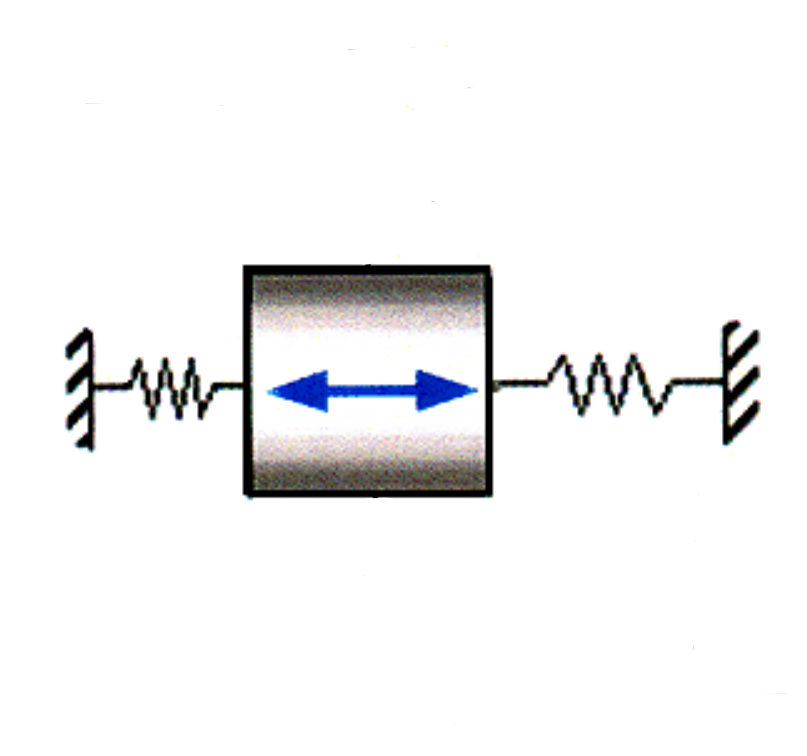
\includegraphics[width=0.8\textwidth]{acc11}
        \end{figure}
        \column{0.5\textwidth}
        \begin{figure}[htpb]
            \centering
            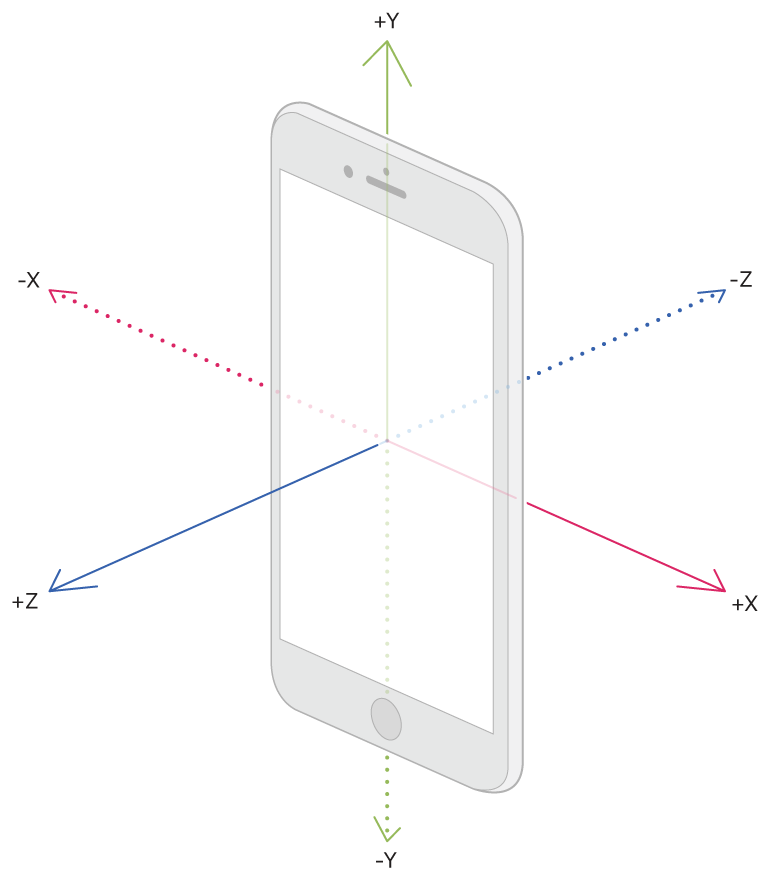
\includegraphics[width=1\textwidth]{acc}
        \end{figure}
    \end{columns}
\end{frame}

\begin{frame}
    \frametitle{Sensor: Beschleunigungssensor Rohdaten vs. Linear}
    \begin{columns}
        \column{0.5\textwidth}
        \begin{itemize}
            \item Handy im freien Fall 
                \begin{align*}
                    a_{y,lin}=1\,g \neq a_{y,roh}=0\,g
                \end{align*}   
            \item Handy in Ruhe 
                \begin{align*}
                    a_{y,lin}=0\,g \neq a_{y,roh}=1\,g
                \end{align*} 
            \item Für die Rohdaten gilt
                \begin{align*}
                    \vec{a}_{\,\text{roh}} = \vec{a}_{\,\text{lin}}+\begin{pmatrix}0\\g\\0 \end{pmatrix}
                \end{align*}
        \end{itemize}
        \column{0.5\textwidth}
        \begin{figure}[htpb]
            \centering
            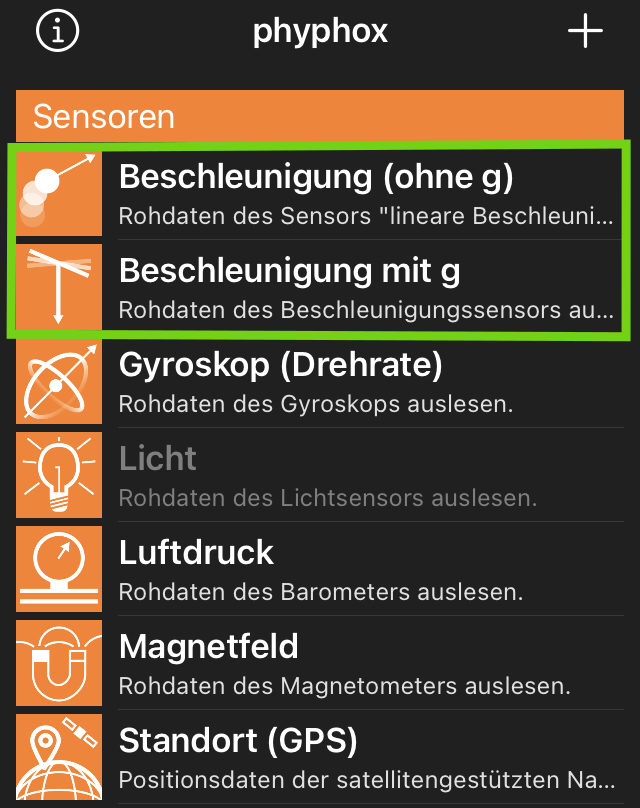
\includegraphics[width=0.9\textwidth]{acc_phyphox}
        \end{figure}
    \end{columns}

\end{frame}

\begin{frame}
    \frametitle{Sensor: Beschleunigungssensor Phyphox}
    \begin{columns}
        \column{0.5\textwidth}
        \begin{center}Beschleunigung mit $g$\end{center}
        \vspace{-0,5cm}        
        \begin{figure}[htpb]
            \centering
            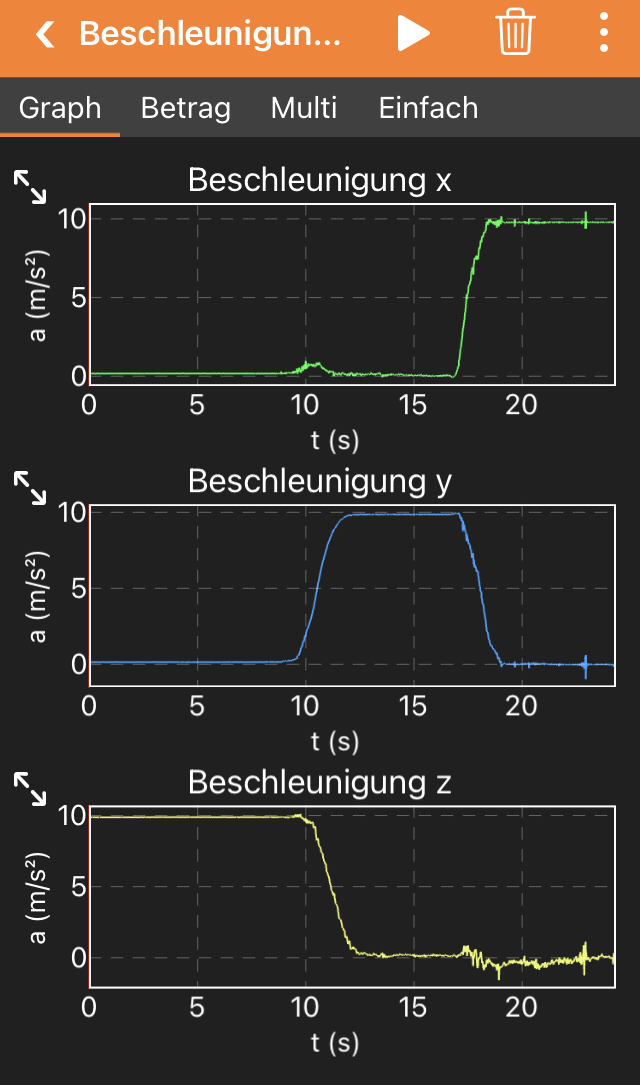
\includegraphics[width=0.8\textwidth]{acc_phyphox2}
        \end{figure}
        \column{0.5\textwidth}
        \begin{center}Beschleunigung ohne $g$\end{center}
        \vspace{-0,5cm}
        \begin{figure}[htpb]
            \centering
            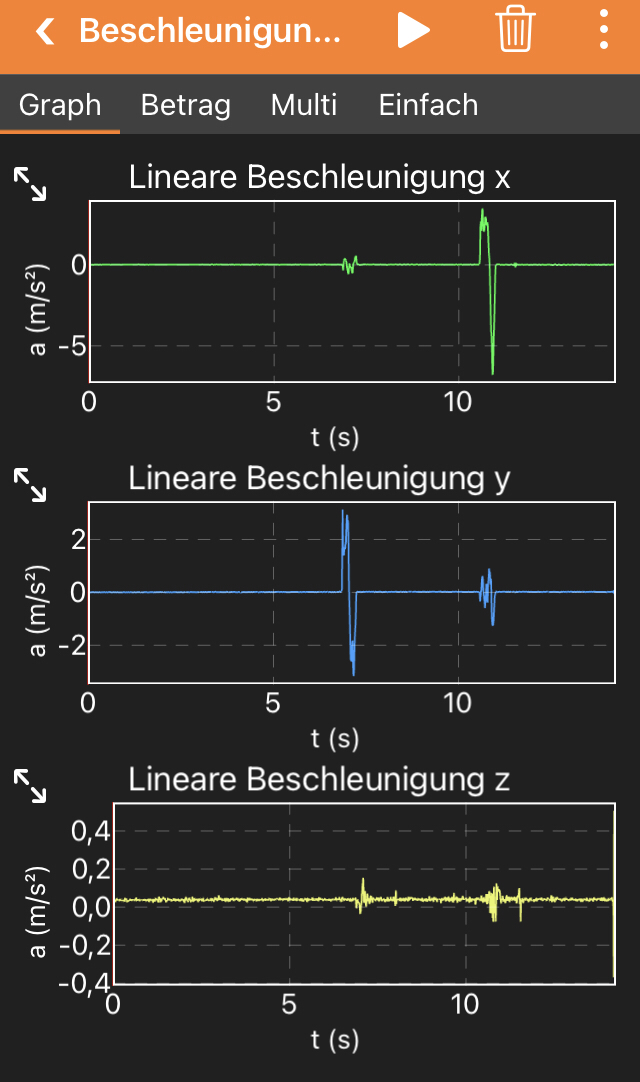
\includegraphics[width=0.8\textwidth]{acc_phyphox3}
        \end{figure}
    \end{columns}
\end{frame}

\begin{frame}
    \frametitle{Fernzugriff und API}
    \begin{columns}
        \column{0.33\textwidth}
        \begin{figure}[htpb]
            \centering
            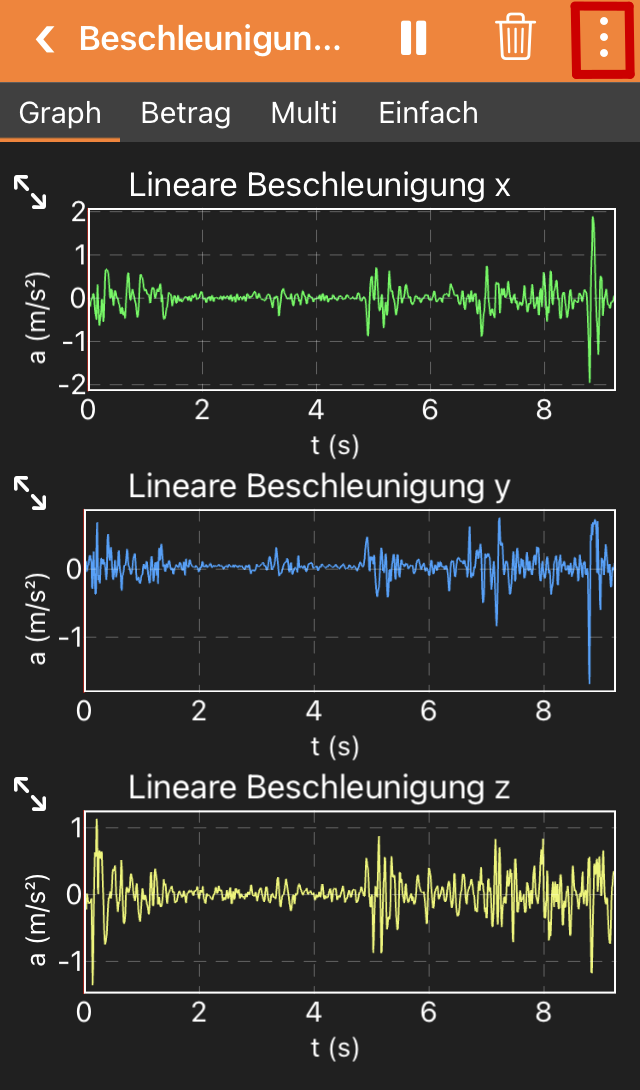
\includegraphics[width=1\textwidth]{fernzugriff1}
        \end{figure}

        \column{0.33\textwidth}
        \begin{figure}[htpb]
            \centering
            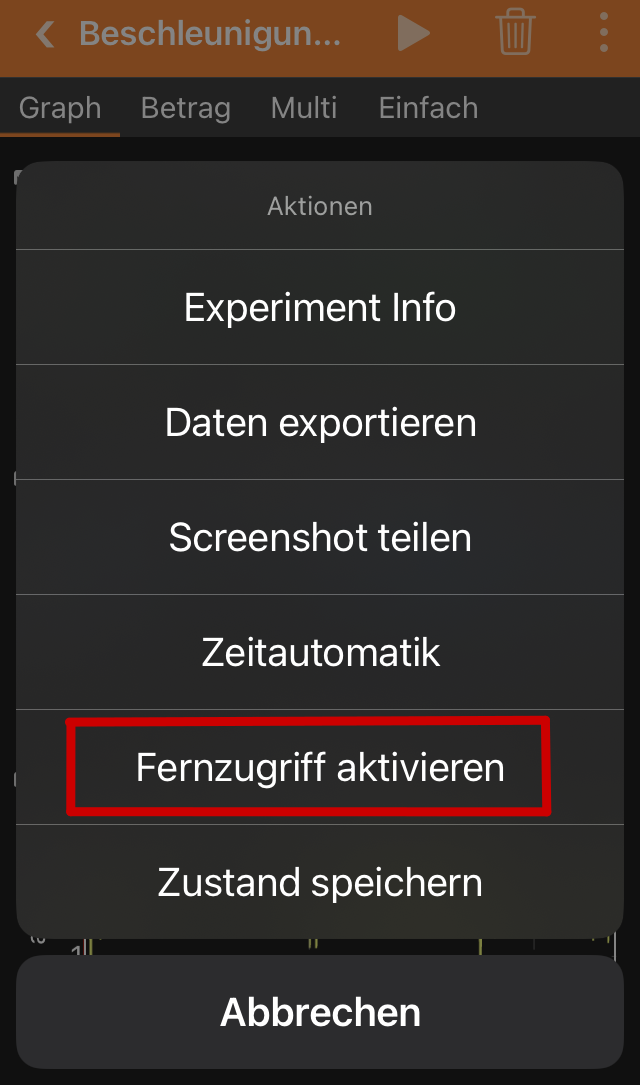
\includegraphics[width=1\textwidth]{fernzugriff2}
        \end{figure}
        \column{0.33\textwidth}
        \begin{figure}[htpb]
            \centering
            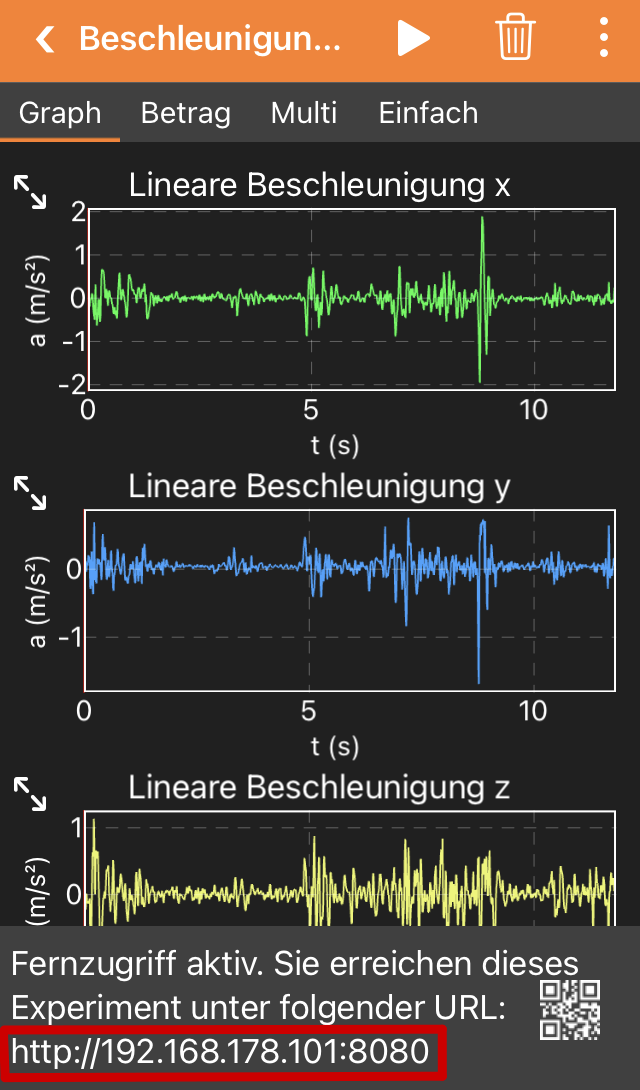
\includegraphics[width=1\textwidth]{fernzugriff3}
        \end{figure}
    \end{columns}

\end{frame}

\begin{frame}
    \frametitle{Versuch: Mechanische Schwingung auf Luftkissenfahrbahn}
    Die Differentialgleichung der Bewegung lautet
    \begin{align*}
        m\ddot{x} = -Dx \quad \text{mit $D=D_1+D_2$}
    \end{align*}
    Als Lösungsansatz verwendet man
    \begin{align*}
        x(t)=a \cdot \sin(b \cdot t +c) +d
    \end{align*}
    Man erhält
    \begin{align*}
        x(t)=A \cos (\omega_0 t) + B \sin(\omega_0 t) \quad \text{mit $\omega_0=\sqrt{\frac{D}{m}}$}
    \end{align*}
\end{frame}

\begin{frame}
    \frametitle{Sensor: Gyroskop} 
    \begin{columns}
        \column{0.5\textwidth}
        \begin{figure}[htpb]
            \centering
            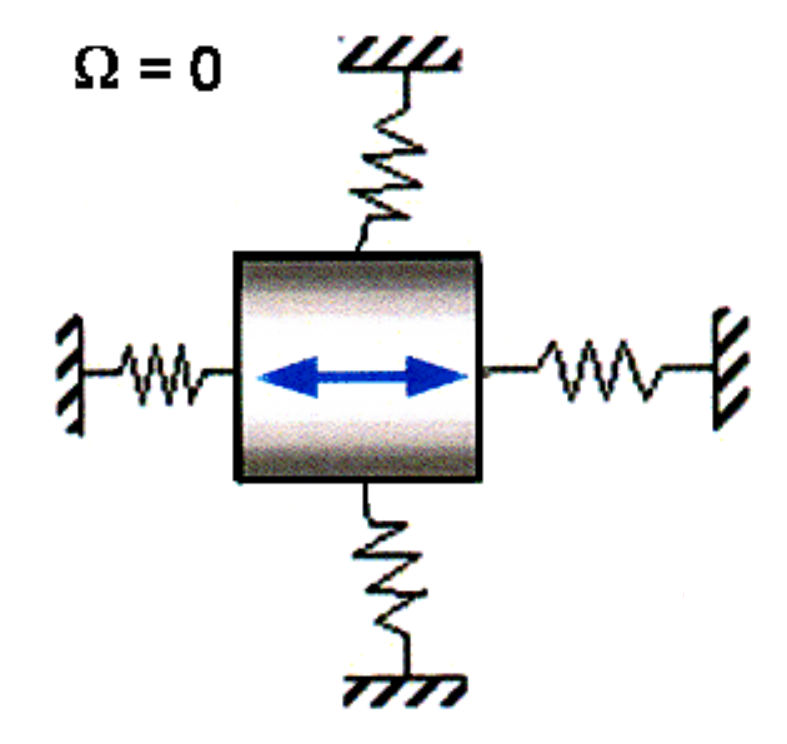
\includegraphics[width=1\textwidth]{gyro8}
        \end{figure}
        \column{0.5\textwidth}
        \begin{figure}[htpb]
            \centering
            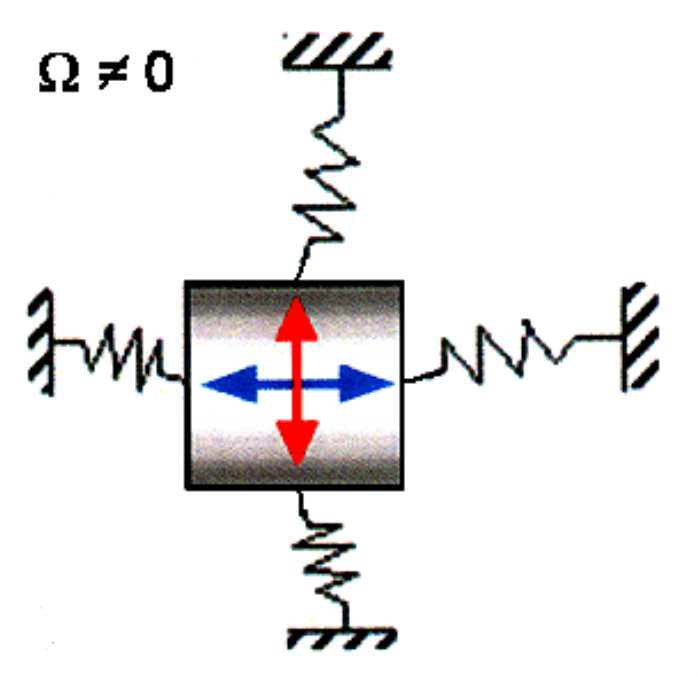
\includegraphics[width=1\textwidth]{gyro7}
        \end{figure}
    \end{columns}
\end{frame}

\begin{frame}
    \frametitle{Sensor: Gyroskop} 
    \begin{figure}[htpb]
        \centering
        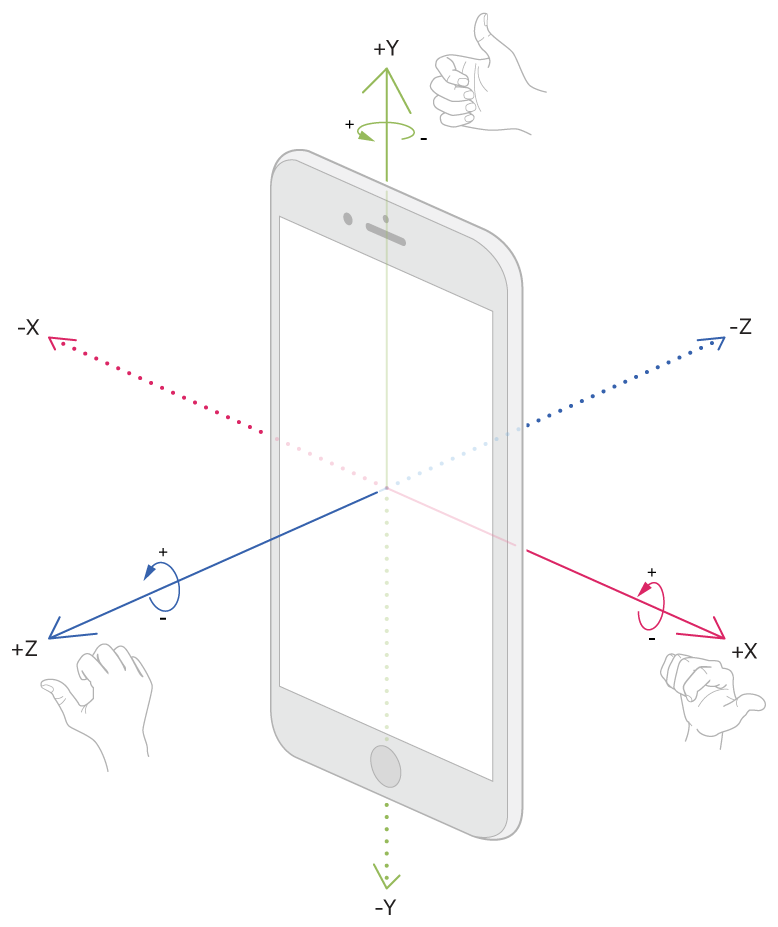
\includegraphics[width=0.6\textwidth]{gyro}
    \end{figure} 
\end{frame}

\begin{frame}
    \frametitle{Sensor: Gyroskop} 
    \begin{columns}
        \column{0.5\textwidth}
        \begin{figure}[htpb]
            \centering
            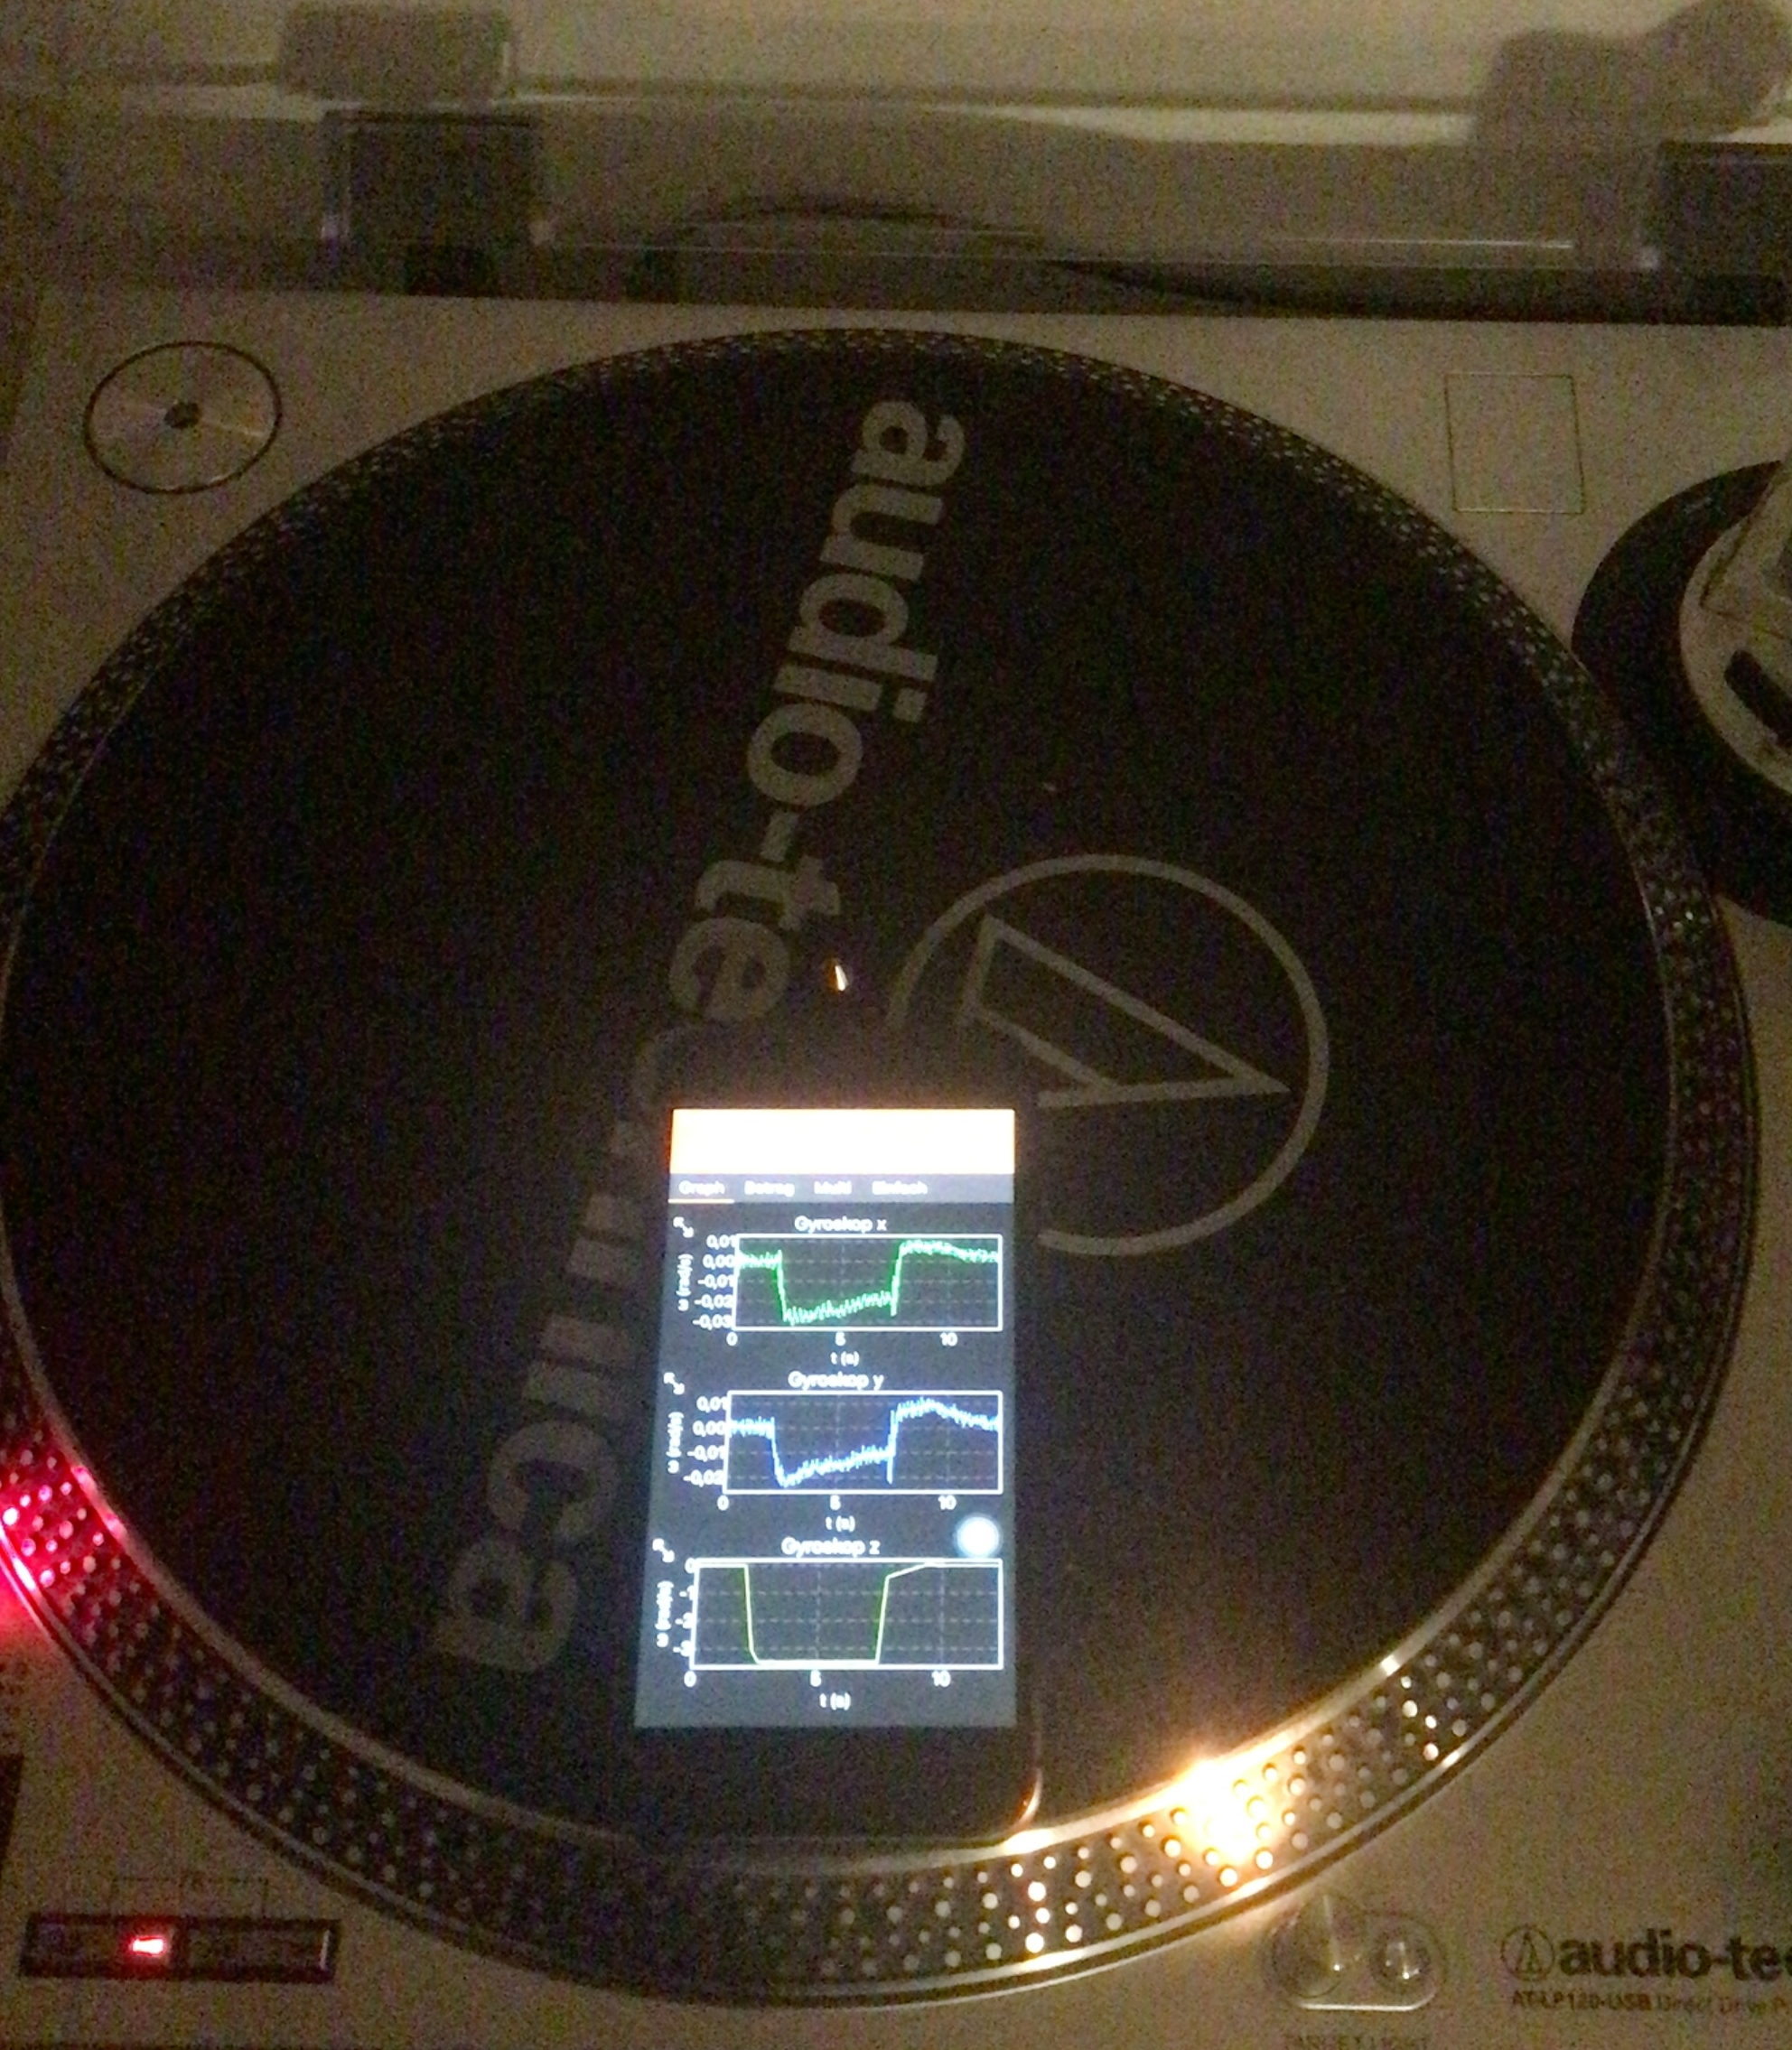
\includegraphics[width=0.8\textwidth]{gyro_turntable}
        \end{figure}
        \column{0.5\textwidth}
        \begin{figure}[htpb]
            \centering
            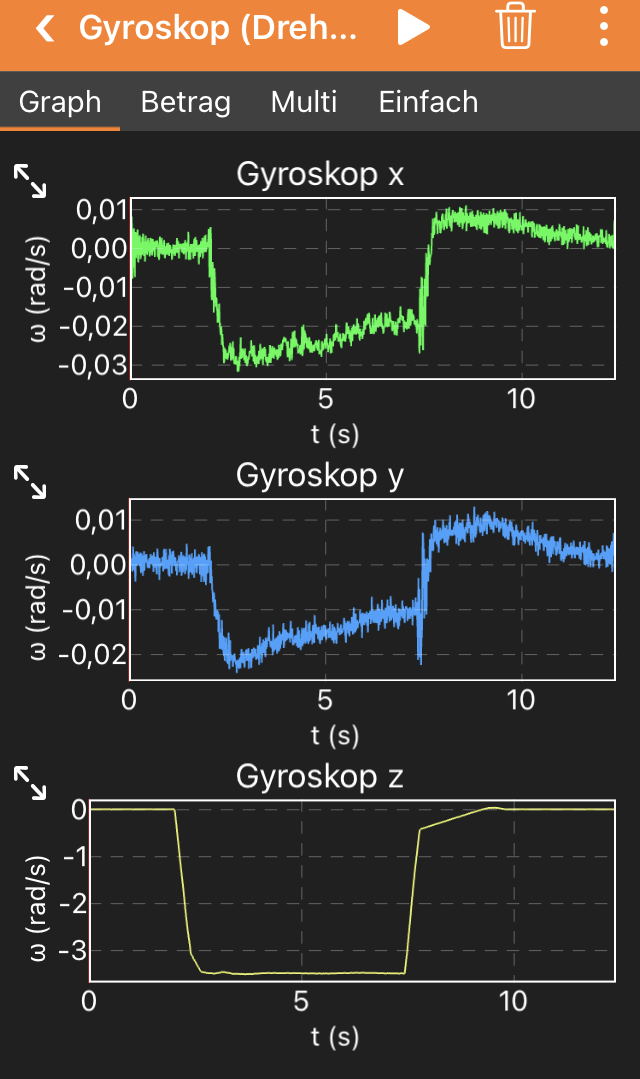
\includegraphics[width=0.6\textwidth]{gyro_turntable2}
        \end{figure}
    \end{columns}
    \begin{align*}
        n \,\, \text{rpm} &\Rightarrow \omega = n \cdot \frac{2\pi}{60\,\text{s}} \approx 0.1 \cdot n \,\, \frac{1}{\text{s}}\\
        33 \,\, \text{rpm} &\Rightarrow \omega \approx 3.3 \,\, \frac{1}{\text{s}}
    \end{align*}
\end{frame}

\begin{frame}
    \frametitle{Versuch: Salatschleuder}
    Bei der Kreisbewegung gilt für die Zentripetalbeschleunigung
    \begin{align*}
        |\vec{a}_{\perp}| = \frac{|\vec{v}|^2}{R} = R \cdot \omega^2 \quad \text{mit} \,\, |\vec{v}|=R\cdot \omega
    \end{align*}
    
\end{frame}

\begin{frame}
    \frametitle{Sensor: Magnetfeldsensor}
    z-Achse zeigt vertikal in Erdoberfläche (z.B. Handy liegt auf einem Tisch):
    \begin{itemize}
        \item Handy nach Norden ausrichten: $B_x \approx 0$
        \item $B_y$ wird größer Richtung Norden und kleiner Richtung Süden
        \item $B_x$ wird größer Richtung Osten und kleiner Richtung Westen
        \item $B_z$ ist negativ Richtung Erdoberfläche und positiv Richtung Himmel
    \end{itemize}
    \begin{figure}[htpb]
        \centering
        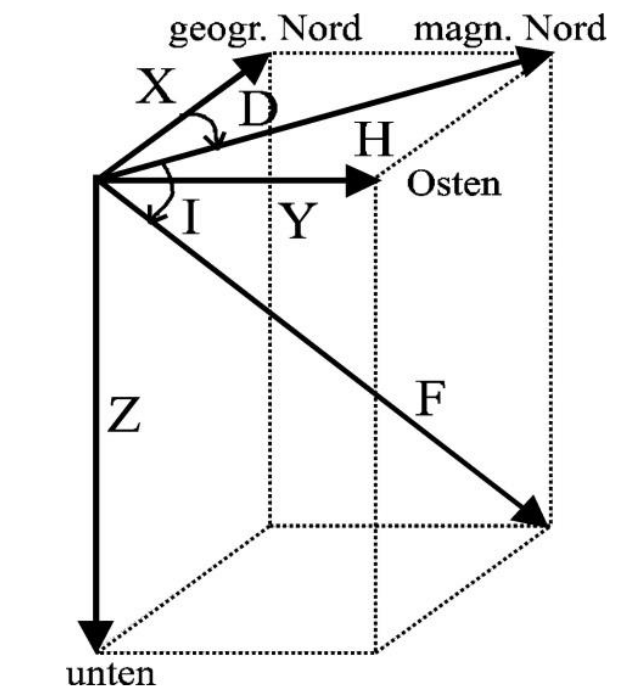
\includegraphics[width=0.3\textwidth]{inklination1}
    \end{figure}
\end{frame}

\begin{frame}
    \frametitle{Versuch: Inklinationskarte}
    \begin{figure}[htpb]
        \centering
        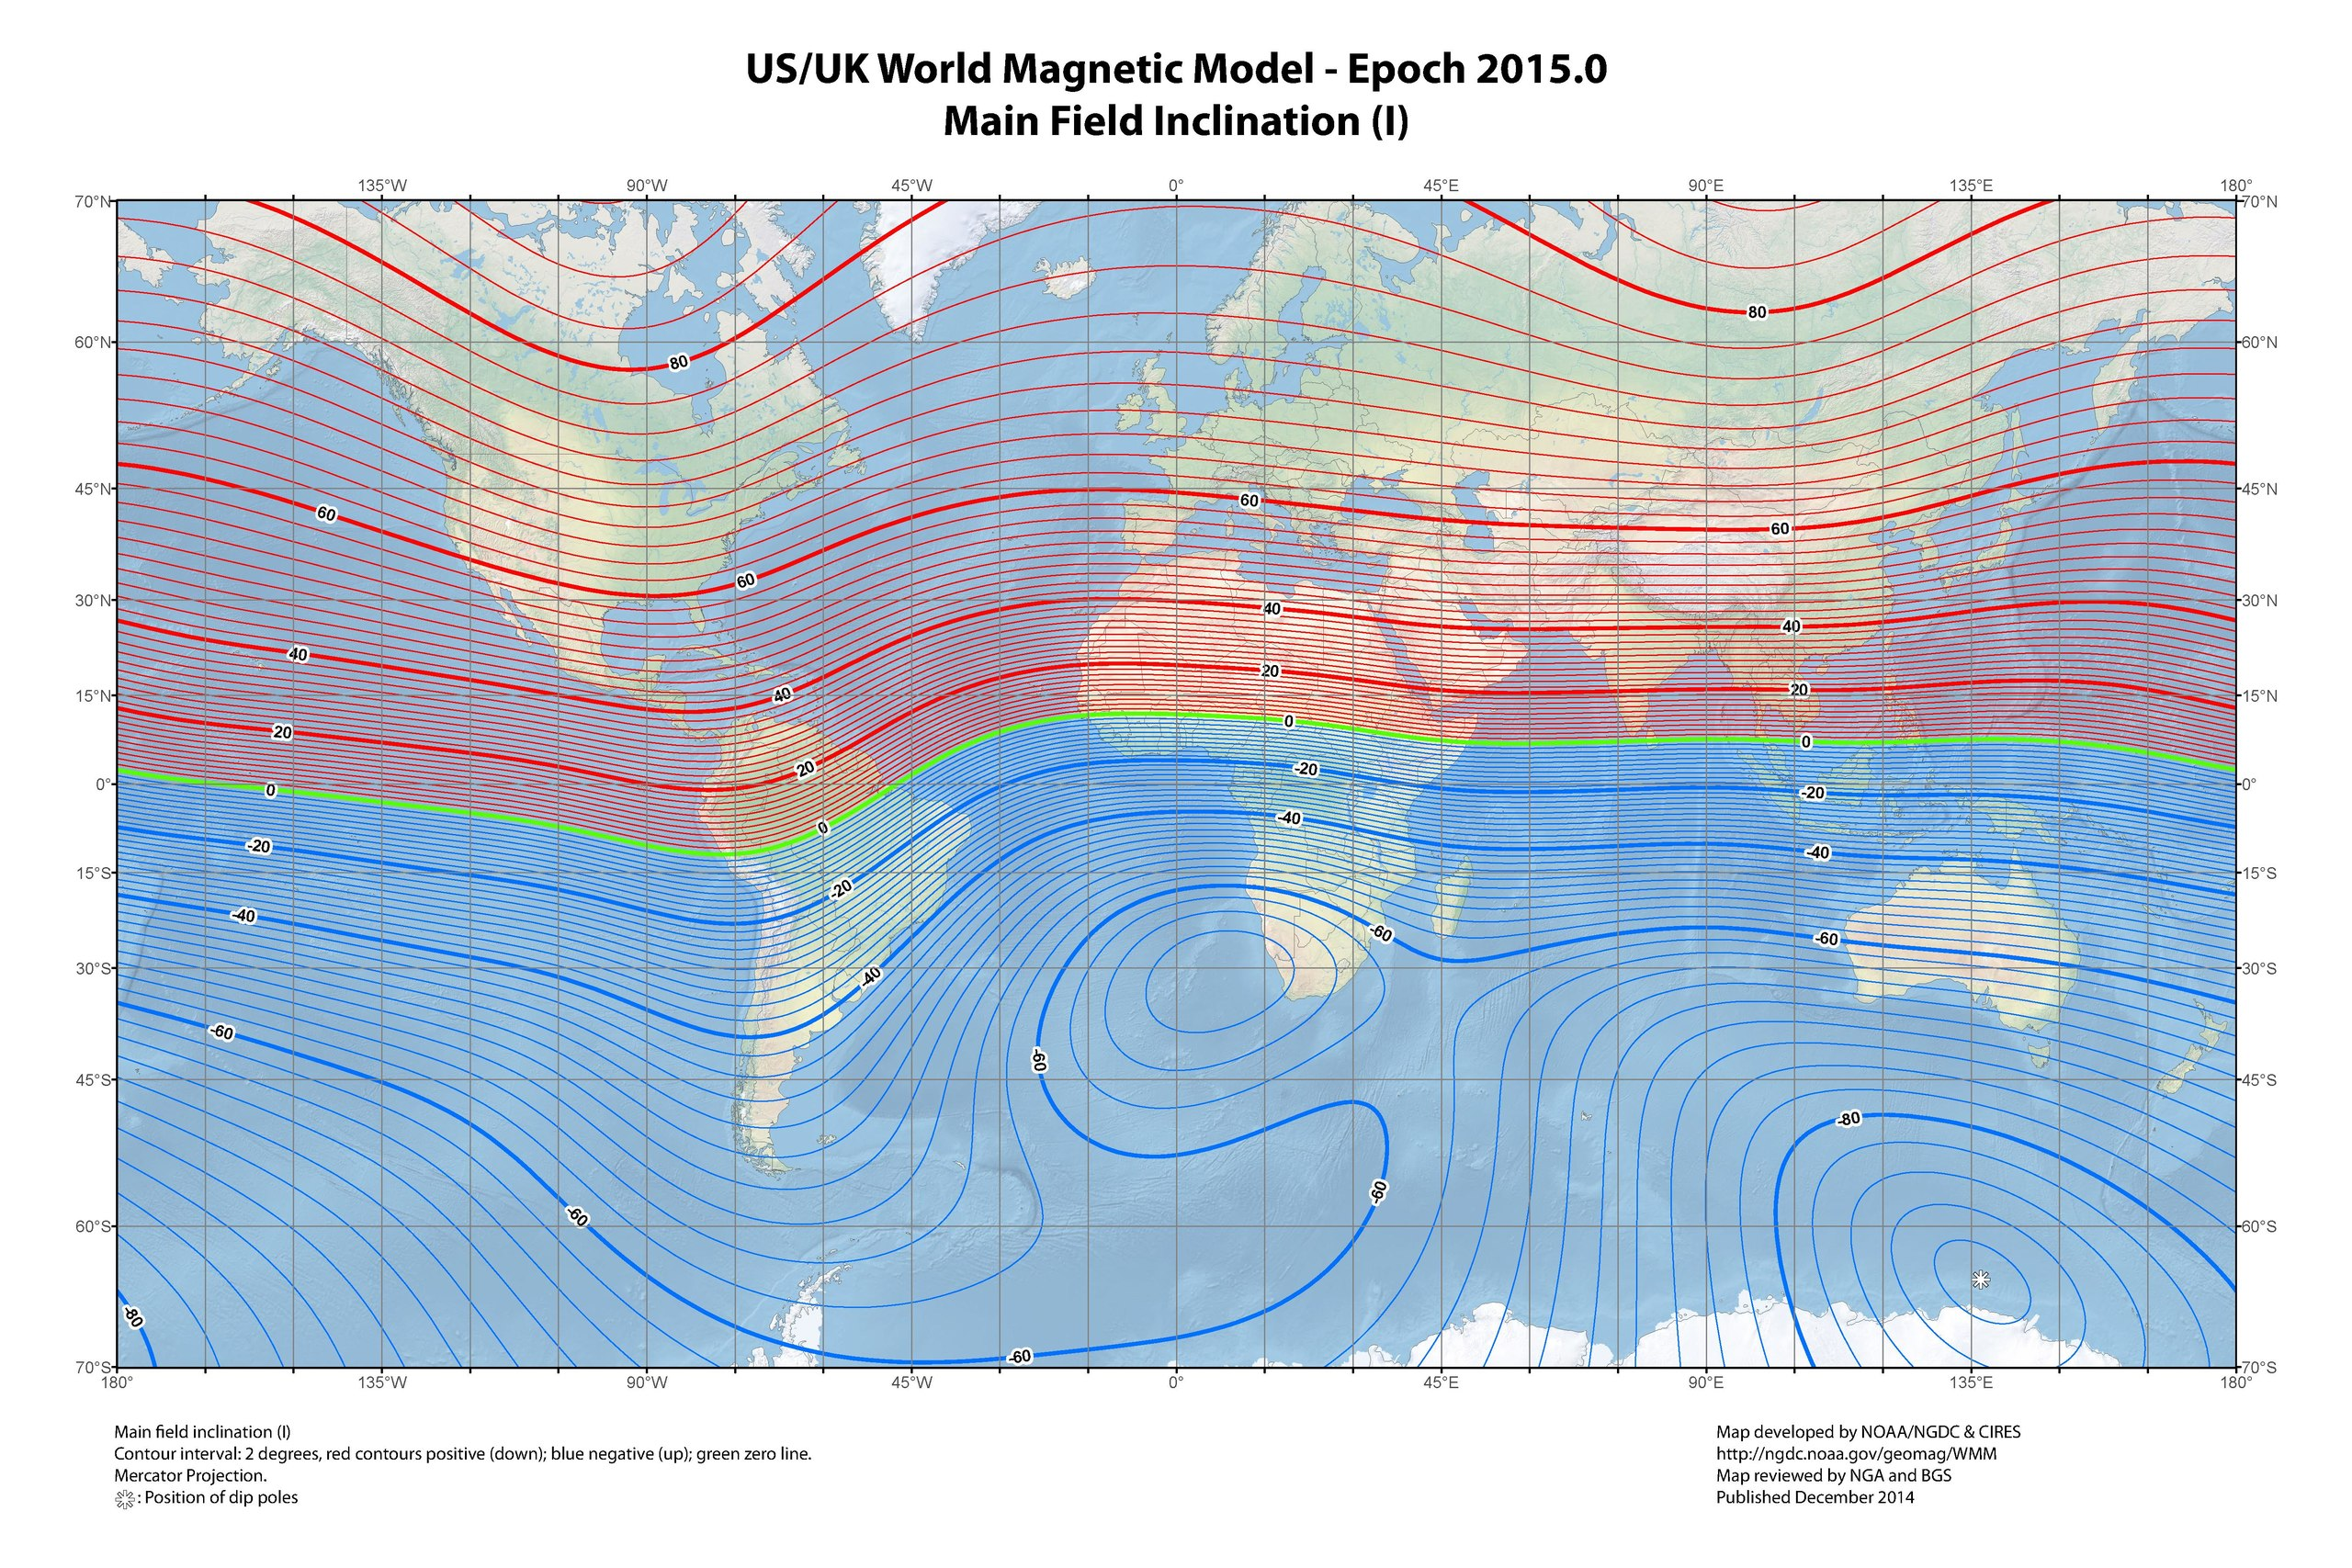
\includegraphics[width=1\textwidth]{inklination2}
    \end{figure}

\end{frame}

\begin{frame}
    \frametitle{Versuch: Fadenpendel}
    \begin{align*}
        T = 2 \pi \sqrt{\frac{l}{g}}
    \end{align*}
    Fragestellungen:
    \begin{itemize}
        \item Einfluss der Masse auf Periodendauer $T$
        \item Einfluss der Startauslenkung auf Periodendauer $T$
        \item Nachweis der Proportionalitäten
        \item Bestimmung der Erdbeschleunigung $g$
    \end{itemize}
\end{frame}

\begin{frame}
    \frametitle{Versuch: Schallgeschwindigkeit}
\end{frame}

\begin{frame}
    \frametitle{Versuch: Schallgeschwindigkeit Festkörper}
    Stab mit freien Enden an beiden Seiten besitzt folgende Eigenfrequenzen von Dehnungsschwingungen:
    \begin{align*}
        \lambda = \frac{2 \cdot L}{n} \Rightarrow f_n = n \cdot \frac{c}{2l} \Rightarrow c=\frac{2lf_n}{n}
    \end{align*}
    \begin{figure}[htpb]
        \centering
        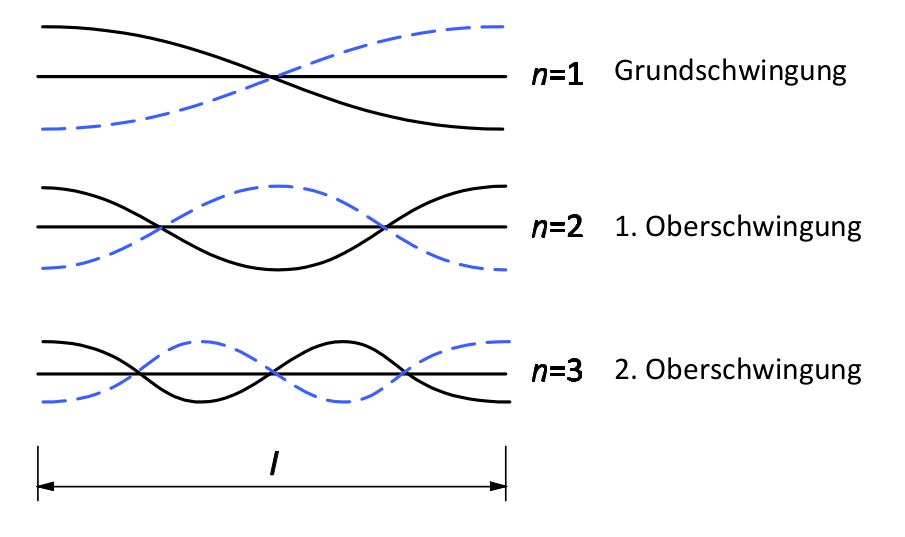
\includegraphics[width=0.8\textwidth]{eigenfrequenzen}
    \end{figure}

\end{frame}

\begin{frame}
    \frametitle{Sensor: Drucksensor}
    In der Regel Anwendung des piezoelektrischen Effekts $\Rightarrow$ Materialien erzeugen elektrisches Signal bei mechanischer Einwirkung
\end{frame}

\begin{frame}
    \frametitle{Versuch: Druckmessung}
\end{frame}
\begin{frame}
    \frametitle{Bluetooth Low Energy (BLE) + Spannungsmessung}
\end{frame}

\begin{frame}
    \frametitle{Versuch: Diode-Kennlinie}
\end{frame}

\begin{frame}
    \frametitle{Versuch: Malus-Gesetz}
    Der Widerstandswert eines Fotowiderstands nimmt linear mit der Intensität der Beleuchtung ab.
    \begin{align*}
        I \uparrow \quad \Rightarrow \quad R \downarrow \quad \Rightarrow \quad U \downarrow \\
        I \downarrow \quad \Rightarrow \quad R \uparrow \quad \Rightarrow \quad U \uparrow \\
    \end{align*}
    
    Gesetz von Malus:
    \begin{figure}[htpb]
        \centering
        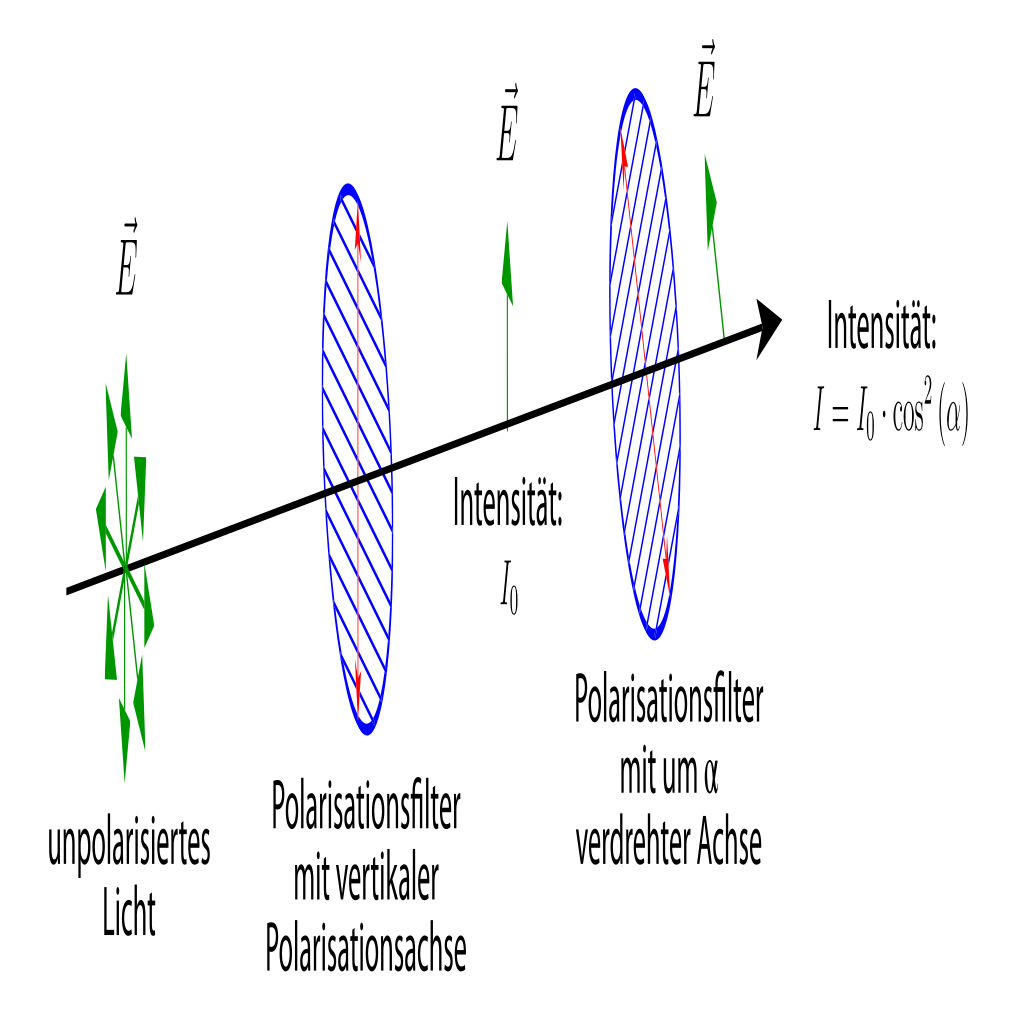
\includegraphics[width=1\textwidth]{malus}
    \end{figure}
\end{frame}

\end{document}
